\documentclass[border=3pt,tikz]{standalone}
\usepackage{tikz}
\usetikzlibrary{positioning}

\begin{document}
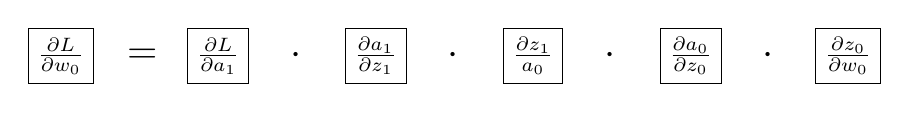
\begin{tikzpicture}[
        dot/.style={
        draw=none,
        font=\Large
    },    
    equals/.style={
        draw=none,
        font=\Large
    }
    ]

    \node[draw] (dloss_0) at (0,0) {$\frac{\partial L}{\partial w_0}$};
    \node[equals, right=3mm of dloss_0] (equals1) {$=$};
    \node[draw] (dloss_1) at (2,0) {$\frac{\partial L}{\partial a_1}$};
    \node[dot, right=4mm of dloss_1] (dot1) {$\cdot$};
    \node[draw] (da_1) at (4,0) {$\frac{\partial a_1}{\partial z_1}$};
    \node[dot, right=4mm of da_1] (dot2) {$\cdot$};
    \node[draw] (dz_1) at (6,0) {$\frac{\partial z_1}{a_0}$};
    \node[dot, right=4mm of dz_1] (dot3) {$\cdot$};
    \node[draw] (dz_0) at (8,0) {$\frac{\partial a_0}{\partial z_0}$};
    \node[dot, right=4mm of dz_0] (dot4) {$\cdot$};
    \node[draw] (dz_0) at (10,0) {$\frac{\partial z_0}{\partial w_0}$};
\end{tikzpicture}
\end{document}
